\documentclass{beamer}%[handout] slides non ripetute

\usetheme{Singapore}
\usecolortheme{rose}

\usepackage[utf8]{inputenc}	%lettere accentate
\usepackage[italian]{babel}	%sillabazione italiana
\usepackage{amsmath}		%simboli matematici
\usepackage{amsfonts}		%font matematici
\usepackage{amssymb}		%altri simboli matematici
\usepackage{tikz}			%grafica
\usepackage{subfloat}		%affiancare figura
\usepackage{cancel}			%simbolo di semplificazione
\usepackage{pdfpages}		%incorporare pdf
\usepackage{biblatex}		%bibliografia
\usepackage{soul}			%testo barrato

\newcommand{\tblue}[1]{\textcolor{blue}{#1}}

\author{Marco Buracchi}

\title{Algoritmi crittografici a chiave condivisa: da Giulio Cesare ai giorni nostri}

\logo{
\includegraphics[scale=0.5]{logo/logoDX0.eps}}

\institute{Università degli studi di Firenze}

\date{\today}

\subject{Security engineering}

%\setbeamercovered{transparent}

\setbeamertemplate{navigation symbols}{}
\setbeamertemplate{caption}[numbered]
\setbeamerfont{caption}{size=\scriptsize}

\begin{document}
	
	\maketitle
	
	\section{Intro}

	\begin{frame}
		\begin{center}
			\LARGE{\tblue{Concetti introduttivi}}
		\end{center}
	\end{frame}

	\subsection{Concetti introduttivi}
	
		\begin{frame}
			\frametitle{Terminologia base}		
			I cinque ingredienti principali con cui lavoreremo sono:
			\begin{itemize}
				\item \tblue{Plaintext}: il messaggio originale da cifrare
				\item \tblue{Ciphertext}: il messaggio cifrato
				\item \tblue{Algoritmo di encryption}: l'algoritmo utilizzato per criptare il plaintext
				\item \tblue{Algoritmo di decryption}: l'algoritmo utilizzato per decriptare il ciphertext
				\item \tblue{Chiave segreta}: la chiave condivisa dalle parti fornita in input all'algoritmo di encryption
			\end{itemize}
		\end{frame}
		
		\begin{frame}
			\frametitle{Crittografia}		
			I sistemi crittografici sono generalmente classificati secondo tre dimensioni:
			\begin{itemize}
				\item Il tipo di operazioni effettuate sul plaintext (sostituzione o trasposizione)
				\item Il numero di chiavi usate
				\item Come il plaintext viene processato (blocchi o stream)
			\end{itemize}
		\end{frame}
	
		{\fontsize{10}{0}
		\begin{frame}
			\frametitle{Principi di Kerckhoffs}	
			Nel 1883 Auguste Kerckhoffs pubblicò ne \tblue{"La Cryptographie Militaire"} i principi progettuali per i cifrari militari	
			\begin{itemize}
				\item Il sistema deve essere praticamente, se non matematicamente, indecifrabile
				\item \tblue{Questo non deve essere segreto, deve essere in grado di cadere nelle mani del nemico senza inconvenienti}
				\item La sua chiave deve essere comunicabile senza l'aiuto di note scritte, e modificabile o modificabili a piacimento dei corrispondenti
				\item \textst{Deve essere applicabile alla corrispondenza telegrafica}
				\item \textst{Deve essere portatile} e il suo utilizzo non deve richiedere il concorso di più persone
				\item È necessario che la sua applicazione sia facile da usare e che non richieda la conoscenza e l'uso di una lunga serie di regole	
			\end{itemize}
		\end{frame}}
		
		\begin{frame}
			\frametitle{Tipi di attacchi di criptoanalisi possibili}		
			\begin{figure}
				\begin{center}
						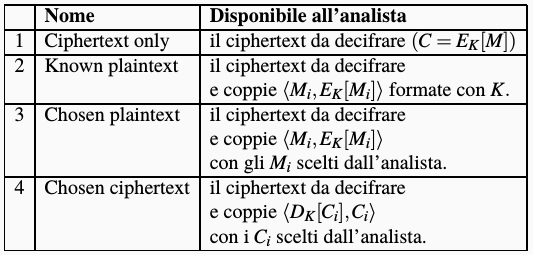
\includegraphics[scale = 0.45]{img/attacchi}
						\caption{Attacchi}
				\end{center}
			\end{figure}
		\end{frame}


	\section{Monoalfabetici}

	\begin{frame}
		\begin{center}
			\LARGE{\textcolor{blue}{Cifrari a sostituzione monoalfabetici}}
		\end{center}
	\end{frame}

	\subsection{Intro}
		
		\begin{frame}
			\frametitle{Shift Encryption}		
			\begin{itemize}
				\item La \textcolor{blue}{encryption} viene eseguita lettera per lettera
				\item Ogni lettera viene sostituita con un'altra lettera (\tblue{fissata})
				\item Identifichiamo le lettere con i \textcolor{blue}{numeri} da 0 a 25 (A=0, B=1, ecc)
				\item Chiamiamo K la chiave segreta che sarà un \textcolor{blue}{numero} compreso tra 1 e 25
				\item Le \textcolor{blue}{funzioni di encryption e decryption} saranno le seguenti
					$$\begin{cases}
						c = E_K[p] = (p+K) mod 26 \\
						p = D_K[c] = (c-K) mod 26
					\end{cases}$$
			\end{itemize}
		\end{frame}
		
		\begin{frame}
			\frametitle{Substitution Encryption}		
			\begin{itemize}
				\item \tblue{Facilmente attaccabile} con forza bruta (solo 26 chiavi possibili)
				\item Si risolve utilizzando una \textcolor{blue}{qualunque} permutazione delle lettere (si passa a 26! $\approx 4x10^{26}$ combinazioni)
				\item Nuovo problema: \tblue{analisi delle frequenze}
			\end{itemize}
		\end{frame}
		
		\begin{frame}
			\frametitle{Criptanalisi}		
			\begin{itemize}
				\item Nella lingua italiana le 5 lettere \textcolor{blue}{più frequenti} sono E($12.62\%$), I($11.62\%$), A($10.41\%$), O($8.71\%$) e R($6.70\%$)
				\item Se si ha a disposizione \textcolor{blue}{abbastanza} ciphertext, la frequenza delle lettere che appaiono in questo sarà più o meno la stessa
				\item Si prova a sostituire le lettere del ciphertext con le  lettere che hanno circa la stessa frequenza e con \tblue{pochi} tentativi si trova il plaintext (e la rispettiva \tblue{chiave})
				\item Vediamo un \tblue{esempio}
			\end{itemize}
		\end{frame}
	
		{
			\setbeamercolor{background canvas}{bg=}
			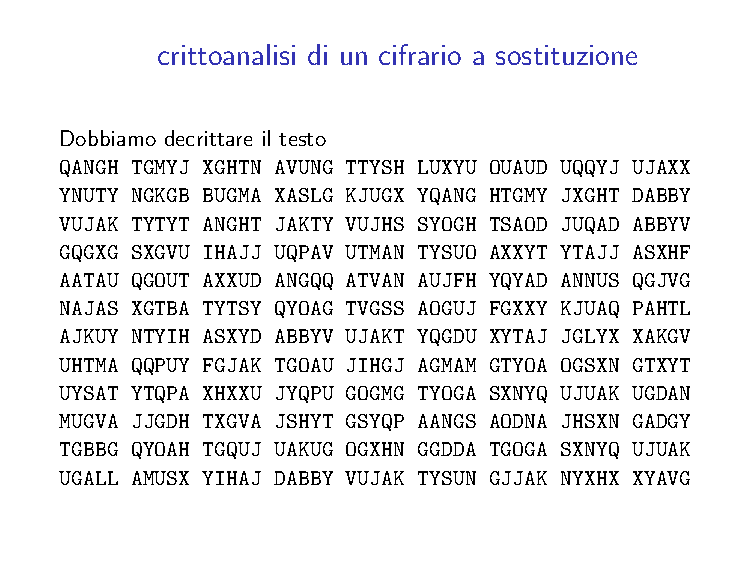
\includepdf[pages={-}]{esempi/cesare.pdf}
		}
					
		\begin{frame}
			\frametitle{Soluzione}		
			\begin{itemize}
				\item Criptare più lettere alla volta (\tblue{cifrari monoalfabetici a blocchi})
				\item Usare più cifrari monoalfabetici a rotazione (\tblue{cifrari polialfabetici})
			\end{itemize}
		\end{frame}
		
	\subsection{Hill}
		
		\begin{frame}
			\begin{center}
				\LARGE{\textcolor{blue}{Cifrari monoalfabetici a blocchi}}
			\end{center}
		\end{frame}
		
		\begin{frame}
			\frametitle{Cenni preliminari}		
			\begin{itemize}
				\item Si lavora con \tblue{\emph{q-grammi}}
				\item La distribuzione dei q-grammi è molto più \tblue{piatta}
				\item Serve \tblue{molto più ciphertext} per effettuare un'analisi delle frequenze significativa
				\item Il cifrario principale in questa categoria è il cifrario di Hill
			\end{itemize}
		\end{frame}
		
		\begin{frame}
			\frametitle{Cifrario di Hill}
			\begin{columns}
				\begin{column}{0.4\textwidth}
					\begin{center}
						\begin{figure}
							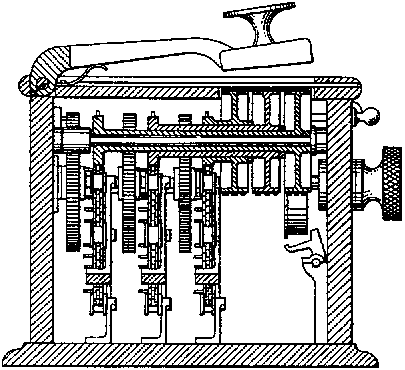
\includegraphics[width=\columnwidth]{img/Hill.png}
							\caption{Macchina cifrante con cifrario di Hill (tratta dal brevetto)}
						\end{figure}	
					\end{center}
				\end{column}
				\begin{column}{0.6\textwidth}
					\begin{itemize}
						\item Creato da \tblue{Lester S. Hill} nel 1929
						\item Si basa sull'utilizzo di \tblue{matrici} e \tblue{algebra modulare}
						\item Si considerano \emph{m} lettere alla volta $p_1,p_2,\dots,p_m$ con \emph{m} \tblue{fissato}.
					\end{itemize}
				\end{column}
			\end{columns}	
		\end{frame}
		
		\begin{frame}
			\frametitle{Encryption}	
			Definiamo:
			$$C = 
			\left(\begin{matrix}
			c_1\\
			\vdots\\
			c_m
			\end{matrix}\right),
			K = 
			\left[\begin{matrix}
			k_{11} & \dots & k_{1m}\\
			\vdots & \vdots & \vdots\\
			k_{m1} & \dots & k_{mm}\\
			\end{matrix}\right],
			P = 
			\left(\begin{matrix}
			p_1\\
			\vdots\\
			p_m
			\end{matrix}\right)$$
			La sostituzione è ottenuta risolvendo il sistema di equazioni lineari:
			$$\begin{cases}
				c_1 = (k_{11}\cdot p_1 + \dots + k_{1m}\cdot p_m)mod 26\\
				\vdots\\
				c_m = (k_{m1}\cdot p_1 + \dots + k_{mm}\cdot p_m)mod 26
			\end{cases}$$	
			In forma matriciale:
			$$E_K[P] = C = KxP$$
		\end{frame}
		
		\begin{frame}
			\frametitle{Decryption}	
			Dal ciphertext si ritorna al plaintext con la formula inversa:
			$$D_K[C] = K^{-1}xC = K^{-1}xKxP = P$$
			Per questo motivo $K$ deve essere \tblue{invertibile} modulo 26.
			\begin{block}{}
				Si sfrutta il principio della \tblue{diffusione} che richiede che ogni lettera del ciphertext dipenda da tutte le lettere del plaintext cosicché le singole lettere del ciphertext non possano essere analizzate singolarmente.
			\end{block}
		\end{frame}
		
		\begin{frame}
			\frametitle{Attacco}	
			Hill è \tblue{vulnerabile} ad un attacco \tblue{known plaintext}.
			
			L'attaccante ha bisogno di \emph{m} coppie di plaintext e rispettivo ciphertext.
			$$\begin{matrix}
				\langle P_1,C_1\rangle & dove \ C_1 = KxP_1\\
				\vdots & \vdots\\
				\langle P_m,C_m\rangle & dove \ C_m = KxP_m
			\end{matrix}$$
			Crea le due matrici 
			$$P^* = \left[P_1|\dots|P_m\right]$$
			$$C^* = \left[C_1|\dots|C_m\right]$$ 
		\end{frame}
		
		\begin{frame}
			\frametitle{Attacco}	
			Sapendo che
			$$C^* = KxP^*(mod 26)$$
			Se $P^*$ è invertibile, calcola l'inversa e può trovare la chiave $K$
			$$C^*xP^{*-1} = KxP^*xP^{*-1} = K$$
			facendo cadere tutto il cifrario.
			Se non lo è, tutto quello che deve fare è raccogliere altre coppie plaintext, ciphertext.
		\end{frame}
	\section{Polialfabetici}

	\begin{frame}
		\begin{center}
			\LARGE{\textcolor{blue}{Cifrari a sostituzione polialfabetici}}
		\end{center}
	\end{frame}

	\subsection{Preliminari}
	
		\begin{frame}
			\frametitle{Idea}		
			\begin{itemize}
				\item Vogliamo \tblue{proteggerci} dall'analisi delle frequenze
				\item In generale vogliamo che due lettere uguali di ciphertext \tblue{non corrispondano} a due lettere uguali di plaintext
				\item Abbiamo bisogno di 
				\begin{itemize}
					\item \tblue{Un insieme} di cifrari monoalfabetici
					\item \tblue{Una regola} per decidere quale cifrario usare per ogni lettera del plaintext 
				\end{itemize}
			\end{itemize}
			\begin{columns}
				\begin{column}{0.2\textwidth}
					\begin{center}
						\begin{figure}
							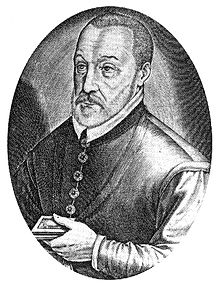
\includegraphics[width=\columnwidth]{img/Vigenere.jpg}
							\caption{Blaise de Vigenère}
						\end{figure}	
					\end{center}
				\end{column}
				\begin{column}{0.8\textwidth}
					\begin{itemize}
						\item Il più famoso cifrario di questo tipo è quello pubblicato nel 1586 dal crittografo francese \tblue{Blaise de Vigenère}
					\end{itemize}
				\end{column}
			\end{columns}
		\end{frame}
	
		\begin{frame}
			\frametitle{Il cifrario}		
			\begin{itemize}
				\item 26 caratteri alfabetici
				\item Sia \emph{m} la lunghezza della chiave $K$, $P_i,C_i,K_i$ la \emph{i-esima} lettera di plaintext, ciphertext e chiave. Per $i = 1,2,\dots$ le funzioni di encryption e decryption sono:
				$$E_K[P_i] = P_i + K_{(i-1\ mod\ m)+1} mod 26$$
				$$D_K[C_i] = C_i - K_{(i-1\ mod\ m)+1} mod 26$$
			\end{itemize}
			\begin{figure}
				\centering
				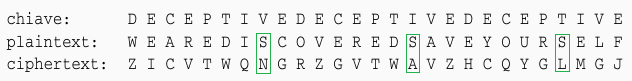
\includegraphics[scale = 0.6]{img/esempiovigenere}
				\caption{Esempio di cifratura}
			\end{figure}
		\end{frame}
		
		\begin{frame}
			\frametitle{Problema risolto? No!}		
			\begin{itemize}
				\item La \tblue{ripetizione} della chiave introduce \tblue{regolarità}
			\end{itemize}
			\begin{figure}
				\centering
				
\includegraphics[scale = 0.5]{img/esempiovigeneredue}
			\end{figure}
			\begin{itemize}
				\item Vediamo come sfruttare questa \tblue{vulnerabilità}
			\end{itemize}
		\end{frame}
	
		{
			\setbeamercolor{background canvas}{bg=}
			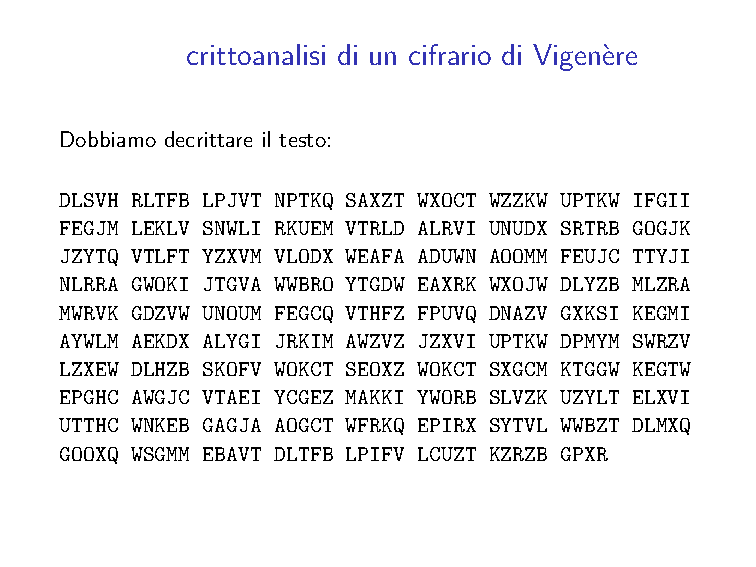
\includepdf[pages={1-3,5,9,11}]{esempi/vigenere.pdf}
		}
	
		\begin{frame}
			\frametitle{Verso One Time Pad}	
			\begin{itemize}
				\item Bisognerebbe poter utilizzare una chiave \tblue{casuale} e \tblue{molto lunga}, possibilmente, tanto quanto il messaggio da trasmettere $\Rightarrow$ \tblue{OneTime Pad}
			\end{itemize}
		\end{frame}
	\section{OTP}

	\begin{frame}
		\begin{center}
			\LARGE{\textcolor{blue}{Il cifrario perfetto: One-Time Pad}}
		\end{center}
	\end{frame}

	\subsection{Cifrari perfetti}
	
	{
		\fontsize{10}{0}
		\begin{frame}
			\frametitle{I cifrari perfetti}
			Siano $P,K,C$ \tblue{variabili aleatorie} su insiemi finiti di valori
			\begin{center}
				$\begin{cases}
					P \text{ prende valori nell'insieme dei plaintext}\\
					K \text{ prende valori nell'insieme delle chiavi}\\
					C \text{ prende valori nell'insieme dei ciphertext}
				\end{cases}$
			\end{center}
			Supponiamo $P$ e $K$ \tblue{indipendenti}.
			\begin{block}{}
				Un cifrario si dice \tblue{perfetto} se
				$$\forall p \in P \text{ e }\forall c \in C \text{ con } Pr(C=c) > 0 \text{ vale che:}$$
				$$Pr(P=p|C=c) = Pr(P=p)$$
			\end{block}
		\end{frame}
	}
	\begin{frame}
		\frametitle{One Time Pad}
		\begin{columns}
			\begin{column}{0.4\textwidth}
				\begin{center}
					\begin{figure}
						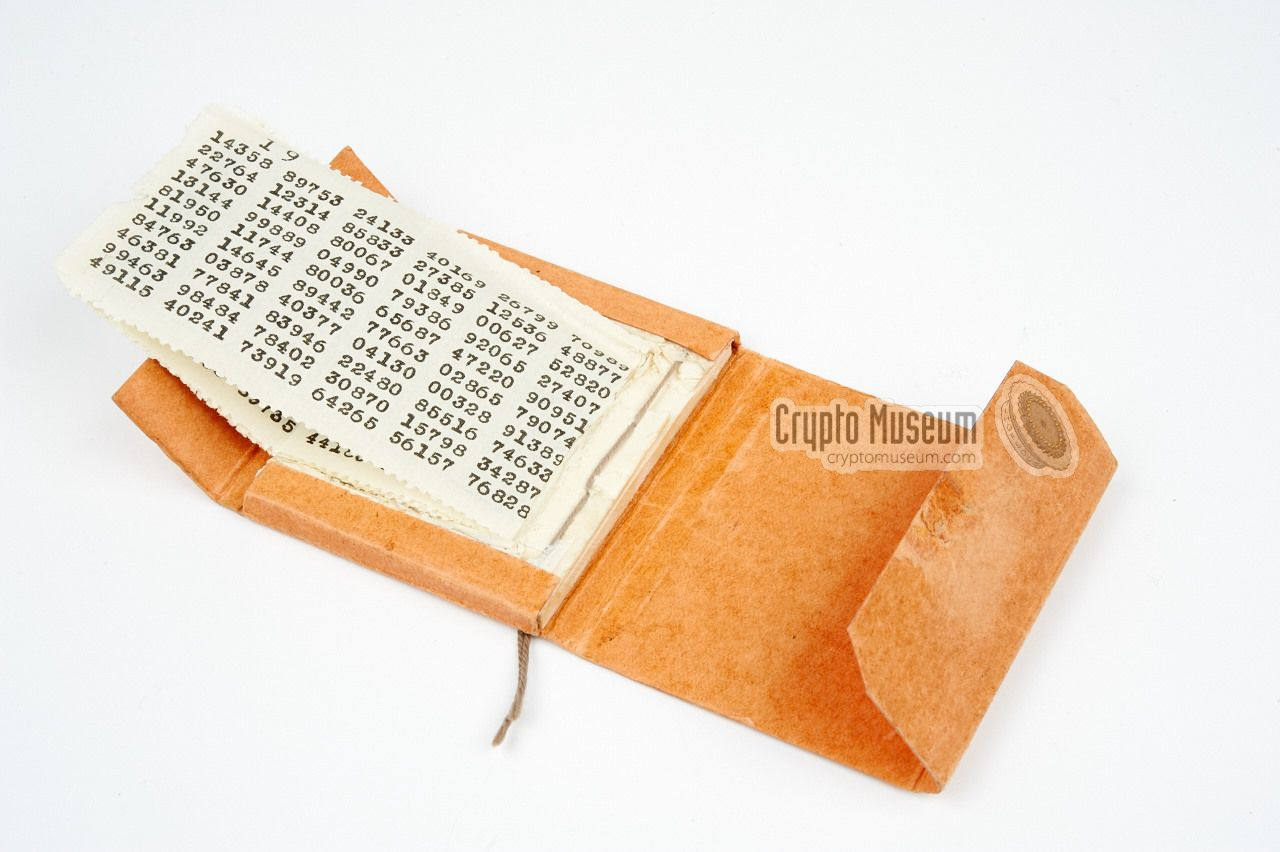
\includegraphics[width=\columnwidth]{img/otp.jpg}
						\caption{One Time Pad sovietico}
					\end{figure}
				\end{center}
			\end{column}
			\begin{column}{0.6\textwidth}
				\begin{itemize}
					\item Introdotto dall'ingegnere dei Bell Labs, \tblue{Gilbert Sandford Vernam} (1890 – 7 febbraio 1960), nel 1926
					\item Il nome deriva dai \tblue{blocchetti} su cui venivano scritte le chiavi
					\item Fissiamo $P = C = K = \{0,1\}^N \text{ con } N>0\text{ \tblue{fissato} e \tblue{noto}}$
					\item Chiave \tblue{perfettamente} casuale $\Rightarrow Pr(K=k)=\frac{1}{2^N}$
				\end{itemize}
			\end{column}
		\end{columns}
	\end{frame}

	\begin{frame}
		\frametitle{One Time Pad}
		Le funzioni di Encryption e di Decryption sono definite come segue:
		$$\begin{cases}
			E_k[p] = p \oplus k = c\\
			D_k[c] = c \oplus k = p \oplus k \oplus k = p
		\end{cases}$$
		{
			\fontsize{10}{0}
			\begin{block}{Esempio}
				$N = 4, P=K=C=\{0,1\}^4$ e supponiamo che i possibili plaintext siano $(0101)$ con probabilità $\frac{3}{4}$ e $(1011)$ con probabilità $\frac{1}{4}$. Se viene scelto $p = (0101) \ e\ k = (1100)$ (che ha probabilità $\frac{1}{2^4}$) otteniamo  $E_k[p] = p \oplus k = (1001) = c$. Lo stesso $c$ è però ottenibile con l'altro $p = (1011)$ e $k = (0010)$. Osservare $c$ come ciphertext non ci permette di risalire con certezza a $p$ senza conoscere $k$.
			\end{block}
		}
	\end{frame}

	\subsection{Dimostrazione}

	\begin{frame}
		\frametitle{One Time Pad}
		\begin{block}{OTP è un cifrario perfetto}
			Supponiamo che ogni $p$ abbia probabilità non nulla di essere generato. Sia $p\in P \ e\ c \in C$ rispettivamente un plaintext e un ciphertext qualsiasi di probabilità non nulla. Dobbiamo dimostrare che $$Pr(P=p|C=c) = Pr(P=p)$$
		\end{block}
	\end{frame}
	\begin{frame}
		\frametitle{One Time Pad}
		$$Pr(P=p|C=c) = \frac{Pr(C=c|P=p)Pr(P=p)}{Pr(C=c)}$$
		Visto che $c = p \oplus k \Leftrightarrow k = c\oplus p$ vuol dire che esiste una \emph{e una sola} chiave $k_{m,c} = c \oplus p$ che permette di cifrare $p$ in $c$ e quindi $$\forall p,c$$ vale che $$Pr(C=c|P=p) = Pr(k_{m,c}) = \frac{1}{2^N}$$ per la distribuzione uniforme delle chiavi.
	\end{frame}
	\begin{frame}
		\frametitle{One Time Pad}
		$$Pr(P=p|C=c) = \frac{\frac{1}{2^N}Pr(P=p)}{Pr(C=c)}$$
		Calcoliamo $Pr(C=c)$ come segue:
		\begin{align*}
			Pr(C=c) &= \sum_{p'\in P}^{}Pr(C=c|P=p')Pr(P=p')\\
			&= \sum_{p'\in P} \frac{1}{2^N}Pr(P=p')\\
			&=\frac{1}{2^N}\sum_{p'\in P}Pr(P=p')\\
			&= \frac{1}{2^N}
		\end{align*}
	\end{frame}
	\begin{frame}
		\frametitle{One Time Pad}
		Da cui si ottiene:
		$$Pr(P=p|C=c) = \frac{\cancel{\frac{1}{2^N}}Pr(P=p)}{\cancel{\frac{1}{2^N}}} = Pr(P=p)$$
	\end{frame}
	\begin{frame}
		\frametitle{Ma allora perché non si usa?}
		\begin{itemize}
			\item Chiave lunga tanto quanto il messaggio
			\item Scala difficilmente con un grande numero di nodi
			\item Sequenze di bit realmente casuali sono difficili da generare
			\item Si stanno studiando metodi quantistici di generazione e distribuzione di chiavi
		\end{itemize}
	\end{frame}

	\section{Enigma}

	\begin{frame}
		\begin{center}
			\LARGE{\textcolor{blue}{Enigma: storia, funzionamento ed analisi}}
		\end{center}
	\end{frame}
	
{ % all template changes are local to this group.
		\setbeamertemplate{navigation symbols}{}
		\begin{frame}[plain]
			\begin{tikzpicture}[remember picture,overlay]
			\node[at=(current page.center)] {
				\includegraphics[scale=0.74]{img/sfondo}
			};
			\end{tikzpicture}
		\end{frame}
	}	
	
	\subsection{Storia}
	
	\begin{frame}
		\frametitle{1918-1923}		
		\begin{itemize}
			\item Il \textcolor{blue}{23 Febbraio 1918}, l'ingegnere tedesco \tblue{Arthur Scherbius}, brevetta una "macchina cifrante a rotori"
			\item Nasce \tblue{ENIGMA}, una delle macchine cifranti più famose della storia
			\item Crea i primi prototipi e tenta di proporla alla milizia tedesca che al momento non è interessata
			\item Decide di fondare una propria azienda per produrre ENIGMA \textcolor{blue}{per scopi commerciali}. 
		\end{itemize}
	\end{frame}
	
	\begin{frame}
		\frametitle{1923-1932}			
		\begin{itemize}
			\item Nel \tblue{1923} vengono messe in commercio le prime macchine
			\item Incorporano una macchina da scrivere, sono \textcolor{blue}{molto pesanti} (circa 50kg) e \textcolor{blue}{poco pratiche} da utilizzare
			\item Non riscossero il successo previsto ma Scherbius continuò a lavorarci per migliorarle
		\end{itemize}
	\end{frame}

	\begin{frame}
		\frametitle{1923-1932}
		\begin{columns}
			\begin{column}{0.45\textwidth}
				\begin{figure}
					\centering
					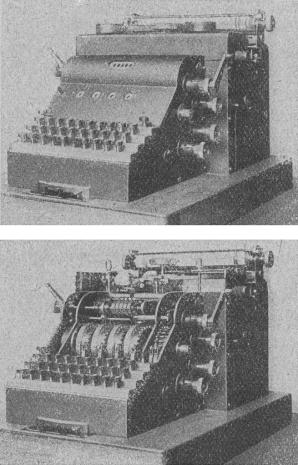
\includegraphics[scale=0.4]{img/A}
					\caption{ENIGMA modello A}
				\end{figure}
			\end{column}
			\begin{column}{0.45\textwidth}
				\begin{figure}
					\centering
					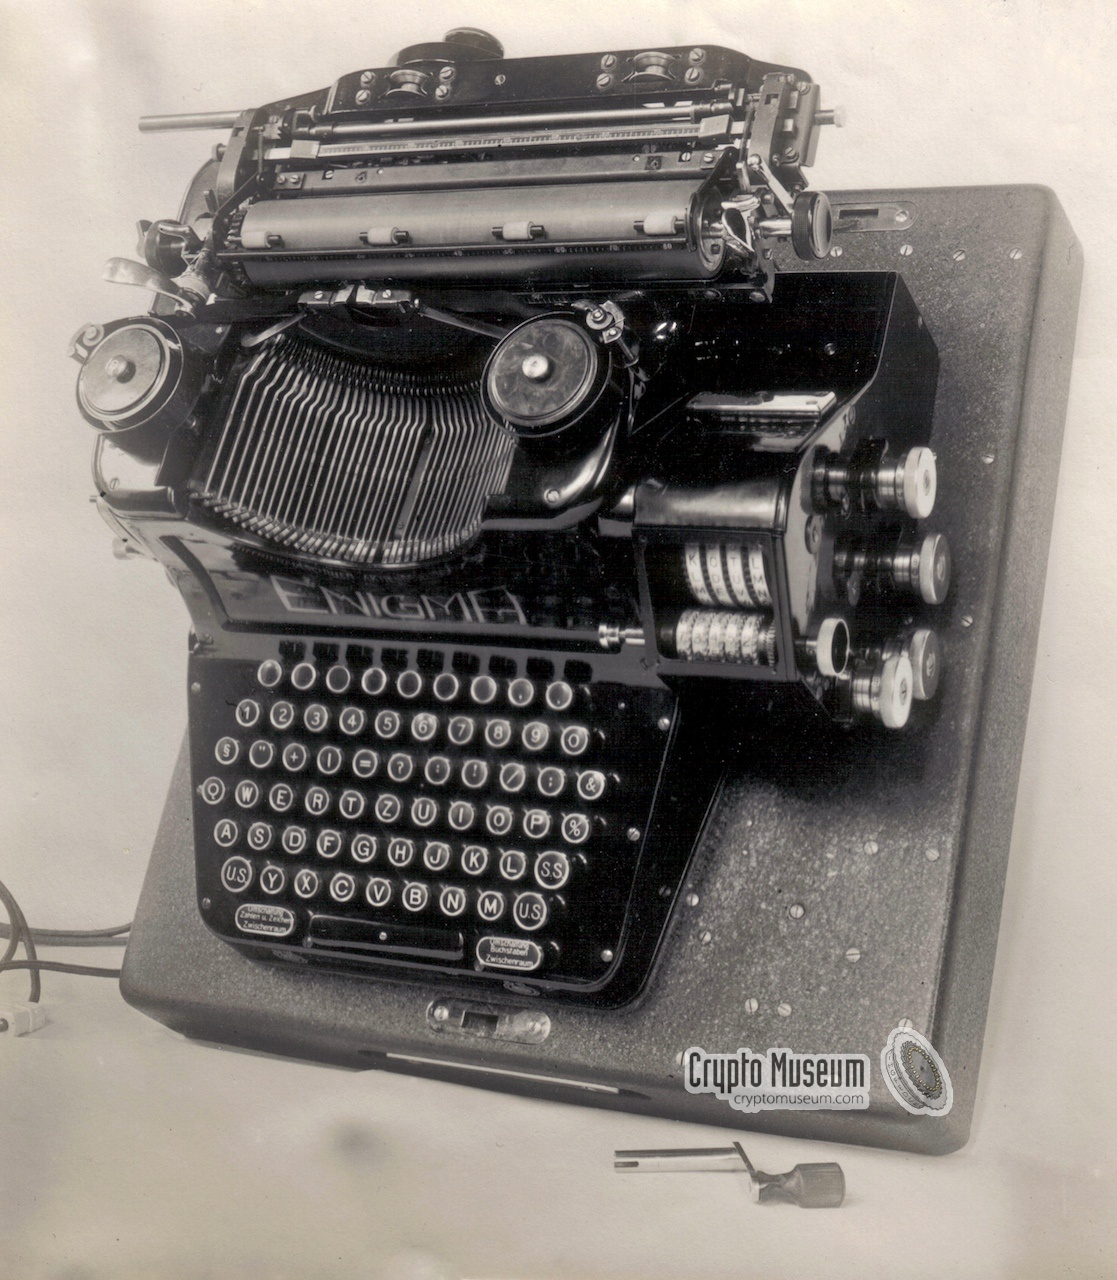
\includegraphics[scale=0.1]{img/B}
					\caption{ENIGMA modello B}
				\end{figure}
			\end{column}
		\end{columns}		
	\end{frame}
	
	\begin{frame}
		\frametitle{1923-1932}		
		\begin{itemize}
			\item Nel \tblue{1925} esce il modello C, il primo a presentare la \textcolor{blue}{lampboard}
			\item La marina si interessa alla macchina e nel \tblue{1926} la adotta ufficialmente (l'esercito lo farà solamente nel \tblue{1928})
			\item Nel \tblue{1932} viene introdotta la \textcolor{blue}{plugboard} e nasce la versione finale di ENIGMA, la \textcolor{blue}{ENIGMA-I}
			\item Da questo momento non è più disponibile in commercio ma viene riservata \textcolor{blue}{esclusivamente} a scopi militari
		\end{itemize}
	\end{frame}
	
	\begin{frame}
		\frametitle{1923-1932}
		\begin{columns}
			\begin{column}{0.45\textwidth}
				\begin{figure}
					\centering
					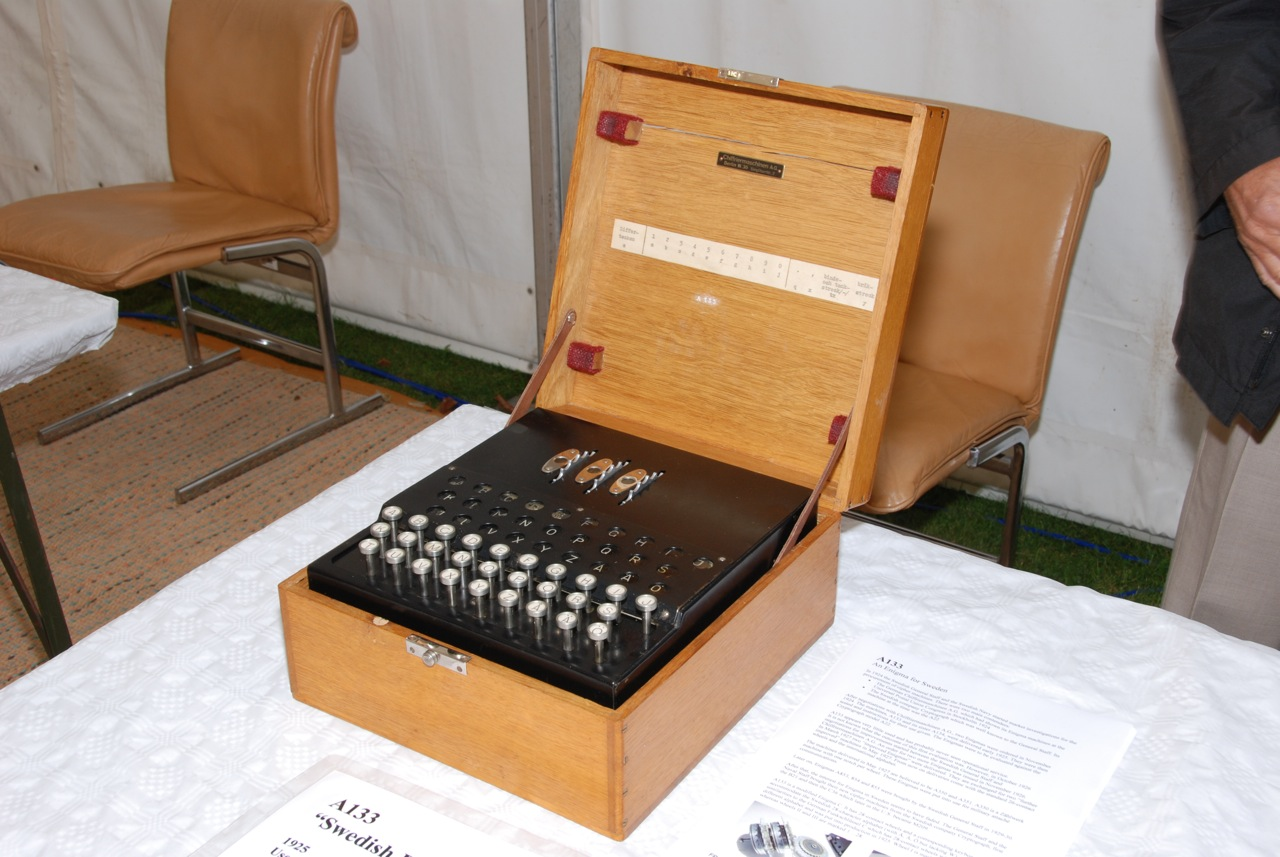
\includegraphics[width=\columnwidth]{img/C}
					\caption{ENIGMA modello C}
				\end{figure}
			\end{column}
			\begin{column}{0.45\textwidth}
				\begin{figure}
					\centering
					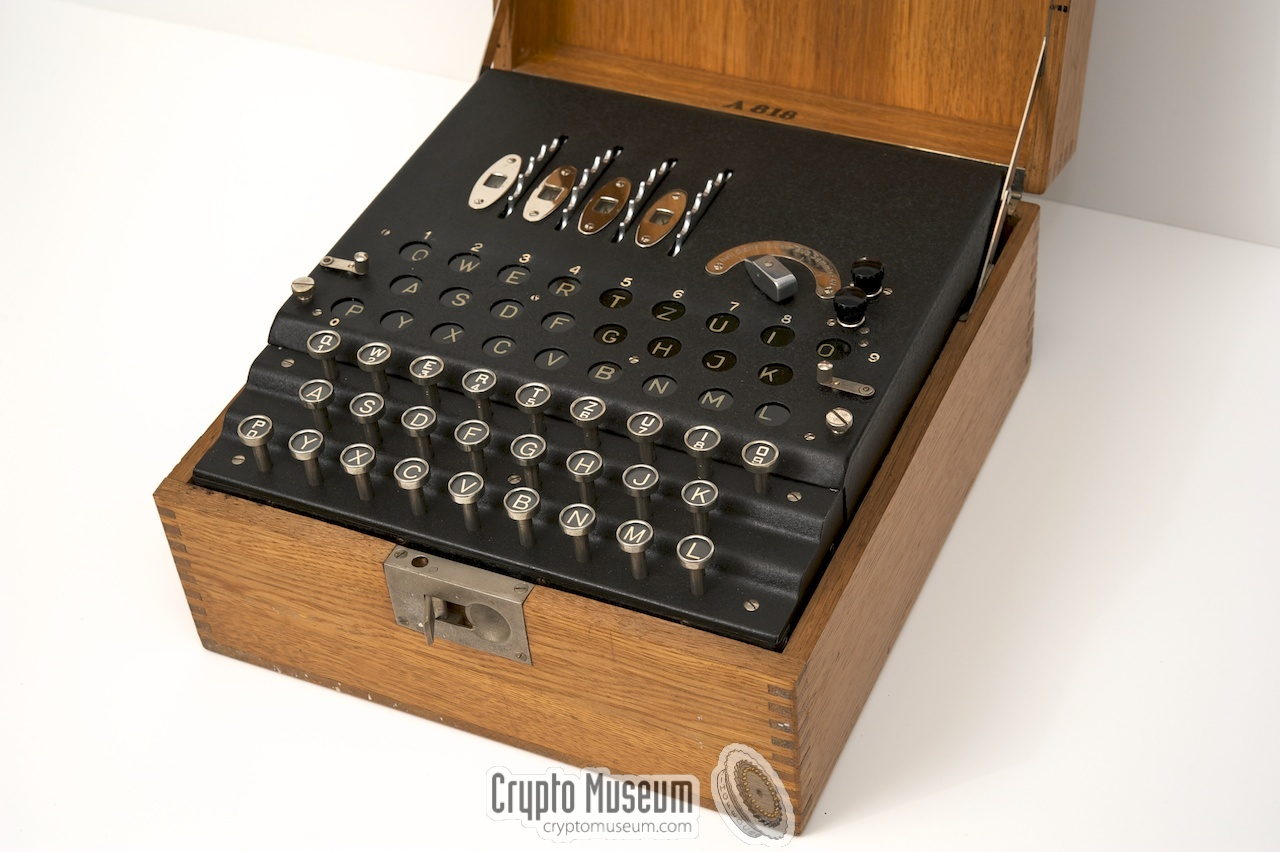
\includegraphics[width=\columnwidth]{img/D}
					\caption{ENIGMA modello D}
				\end{figure}
			\end{column}
		\end{columns}		
	\end{frame}
	
	\begin{frame}
		\frametitle{Dal 1932 alla caduta}		
		\begin{itemize}
			\item La marina e l'esercito \textcolor{blue}{continuano a lavorare su ENIGMA}, adattandola ognuno per i propri scopi e le due macchine presero strade completamente diverse
			\item Nel \tblue{1940} fece la sua apparizione \textcolor{blue}{ENIGMA-M3} l'ultima versione utilizzata dall'esercito per tutta la durata del conflitto.
			\item Da questo momento in avanti, ci riferiremo sempre a questo modello
		\end{itemize}
	\end{frame}
	
	\begin{frame}
		\frametitle{Dal 1932 alla caduta}		
		\begin{figure} [h]
			\centering
			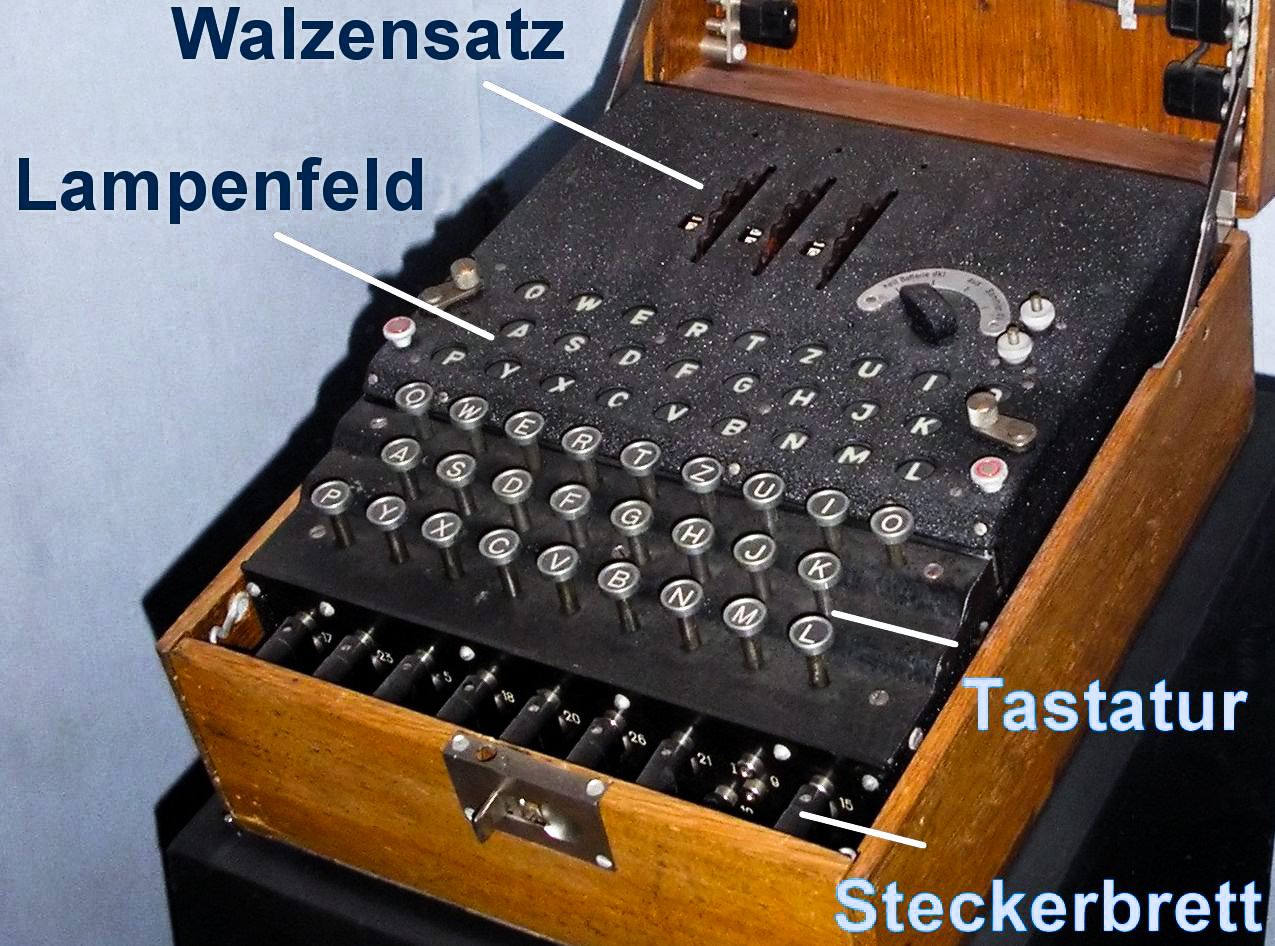
\includegraphics[scale = 0.5]{img/M3}
			\caption{ENIGMA modello M3}
		\end{figure}
	\end{frame}
	
	\subsection{Funzionamento}
	
	\begin{frame}
		\frametitle{Come funziona ENIGMA}
		\begin{itemize}
			\item ENIGMA implementa un \textcolor{blue}{cifrario a sostituzione polialfabetico}
			\item ENIGMA è un dispositivo \textcolor{blue}{elettromeccanico}
			\item Per spiegarne il funzionamento, seguiamo il percorso del \textcolor{blue}{segnale elettrico} al suo interno, dal momento in cui viene premuto un tasto fino all'accensione della lampadina
		\end{itemize}
	\end{frame}
	
	\begin{frame}
		\frametitle{Come funziona ENIGMA}
		\begin{figure}[h]
			\centering
			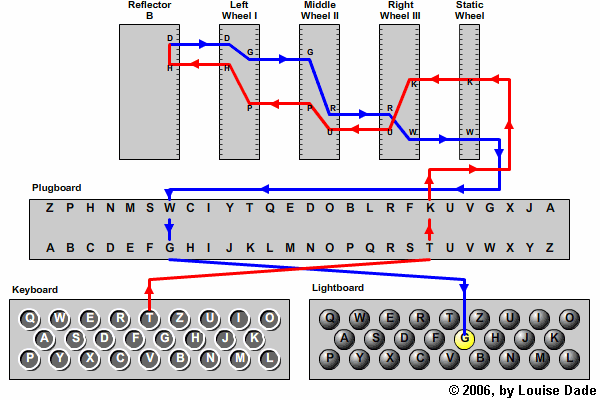
\includegraphics[scale=0.55]{img/wiring}
			\caption{Percorso seguito dal segnale all'interno di ENIGMA}
			\label{fig:wiring}
		\end{figure}
	\end{frame}
	
	\begin{frame}
		\frametitle{Come funziona ENIGMA}
		\begin{itemize}
			\item Analizziamo i vari componenti più in dettaglio
		\end{itemize}
	\end{frame}
	
	\begin{frame}
		\frametitle{Come funziona ENIGMA}
		\begin{figure}
			\centering
			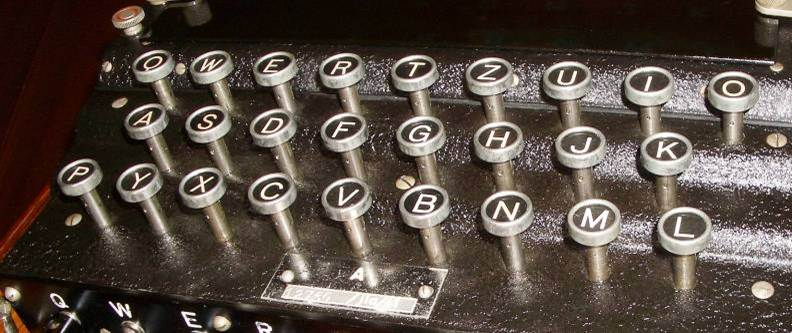
\includegraphics[scale=0.5]{img/keyboard}
			\caption{La tastiera di ENIGMA}
			\label{fig:keyboard}
		\end{figure}
	\end{frame}
	
	\begin{frame}
		\frametitle{Come funziona ENIGMA}
		\begin{figure}[h]
			\centering
			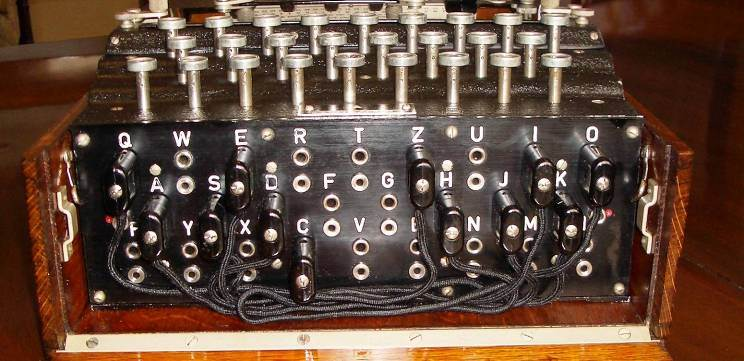
\includegraphics[scale=0.5]{img/plugboard}
			\caption{La plugboard di ENIGMA}
			\label{fig:plugboard}
		\end{figure}
	\end{frame}
	
	\begin{frame}
		\frametitle{Come funziona ENIGMA}
		\begin{columns}
			\begin{column}{0.5\textwidth}
				\begin{center}
					\begin{figure}
						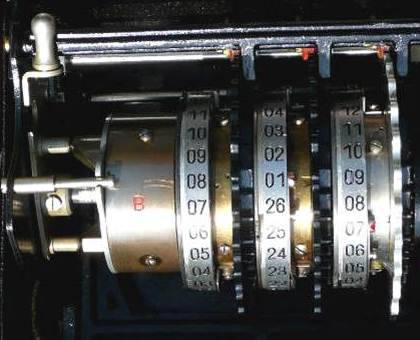
\includegraphics[width=\columnwidth]{img/rotors}
						\caption{Il reflector (a sinistra contrassegnato con una 'B' rossa) e i tre rotori}
					\end{figure}
				\end{center}
			\end{column}
			\begin{column}{0.5\textwidth}
				\begin{center}
					\begin{figure}
						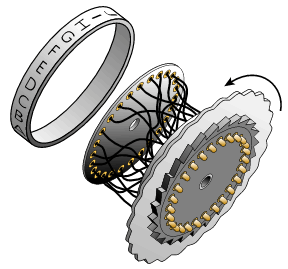
\includegraphics[width=\columnwidth]{img/rotorsexp}
						\caption{Modello di rotore}
					\end{figure}
				\end{center}
			\end{column}
		\end{columns}
	\end{frame}
	
	\begin{frame}
		\frametitle{Come funziona ENIGMA}
		\begin{figure}[h]
			\centering
			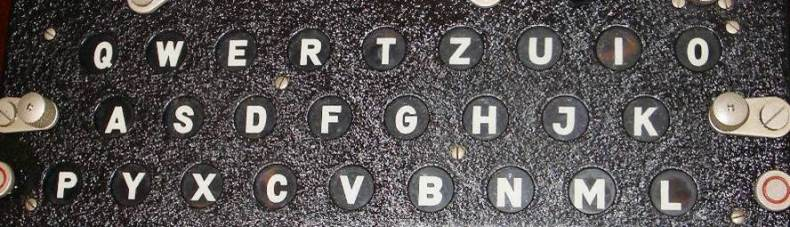
\includegraphics[scale=0.5]{img/lampboard}
			\caption{La lampboard}
			\label{fig:lampboard}
		\end{figure}
	\end{frame}

	\begin{frame}
		\frametitle{La chiave}
		\begin{columns}
			\begin{column}{0.5\textwidth}
				\begin{center}
					\begin{figure}
						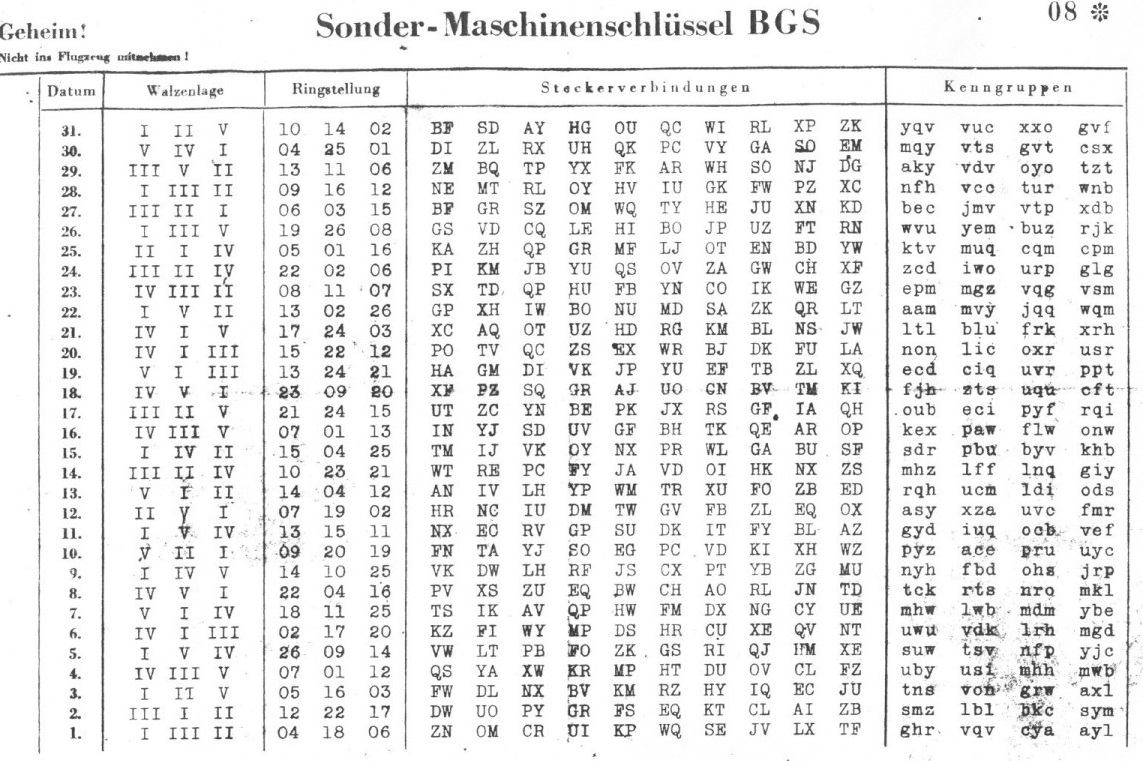
\includegraphics[width=\columnwidth]{img/enigmakeylist}
						\caption{Una pagina del libro delle chiavi}
					\end{figure}
				\end{center}
			\end{column}
			\begin{column}{0.5\textwidth}
				La \tblue{chiave} è formata da:
				\begin{itemize}
					\item I rotori scelti e il loro ordine
					\item La posizione iniziale di ogni rotore
					\item La configurazione della plugboard
					\item Dei caratteri di controllo per risalire alla data del messaggio
				\end{itemize}
			\end{column}
		\end{columns}
	\end{frame}
	
	\subsection{Analisi}
	
	\begin{frame}
		\frametitle{Analisi teorica}
		\begin{itemize}
			\item Configurazione della plugboard
		\end{itemize}
		\begin{figure}[h]
			\centering
			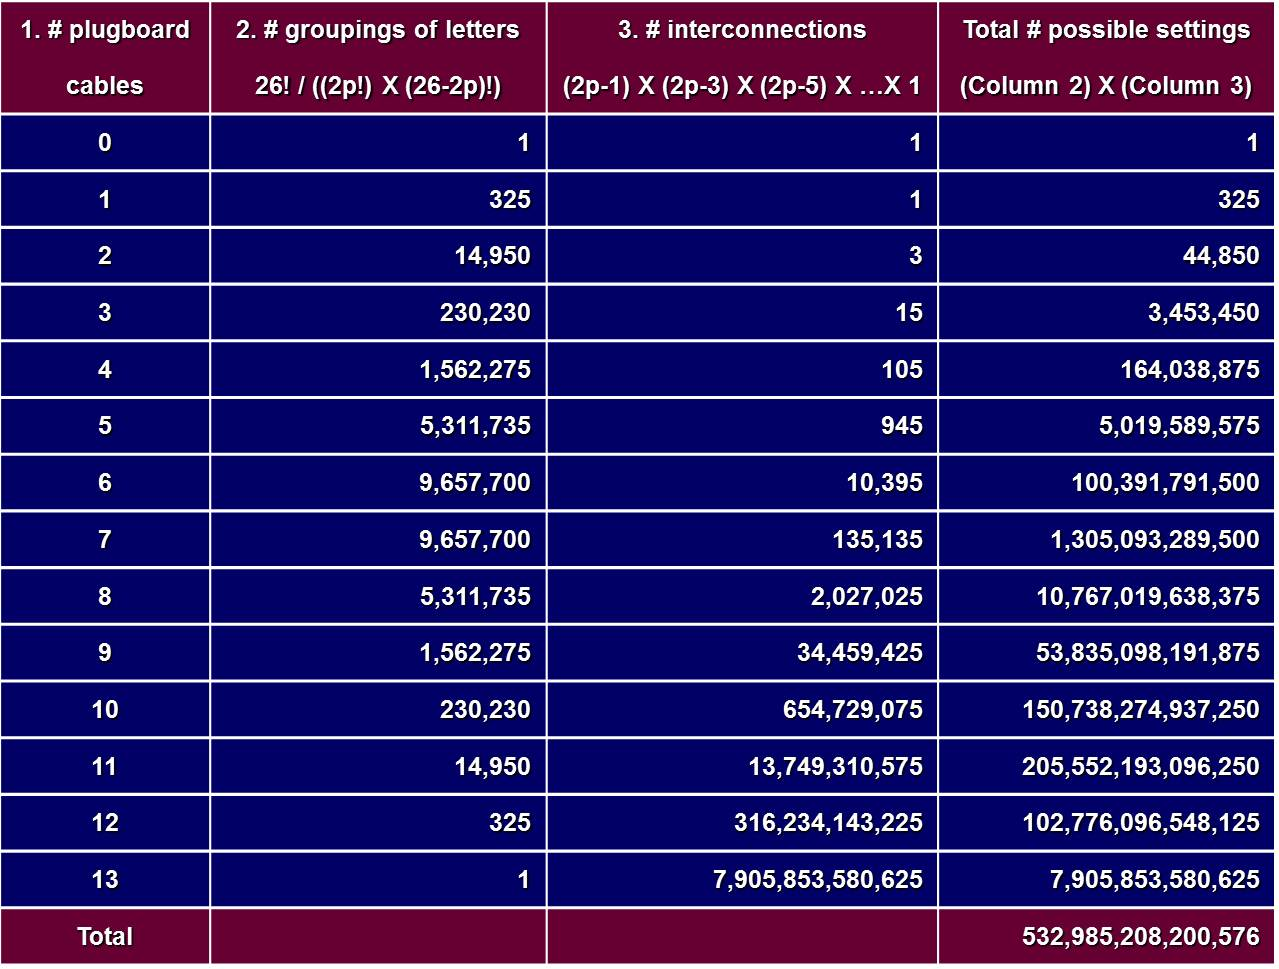
\includegraphics[scale=0.30]{img/plugboardsettings}
			\caption{Criteri possibili della plugboard e conseguenti combinazioni}
			\label{fig:plugboardsettings}
		\end{figure}		
	\end{frame}
	
	\begin{frame}
		\frametitle{Analisi teorica}
		\begin{itemize}
			\item Configurazione dei rotori
			\begin{itemize}
				\item Il cablaggio di ogni rotore poteva essere fatto in \textcolor{blue}{26!} combinazioni differenti
				\item Venivano utilizzati 3 rotori quindi le combinazioni diventano $$26!\cdot(26!-1)\cdot(26!-2)\approx \textcolor{blue}{6.5 \cdot 10^{78}}$$
				\item Ogni rotore poteva essere posizionato inizialmente in una qualunque delle 26 lettere ottenendo altre $\textcolor{blue}{26^3}$ combinazioni
				\item Il rotore più a destra avanza di una lettera ad ogni pressione della tastiera, il secondo e il terzo avanzano di una lettera dopo un giro completo del rotore alla rispettiva destra. Questo apporta ulteriori $(26 \cdot 26)$ \textcolor{blue}{676} combinazioni
			\end{itemize}
		\end{itemize}
	\end{frame}
	
	\begin{frame}
		\frametitle{Analisi teorica}
		\begin{itemize}
			\item Configurazione del reflector
			\begin{itemize}
				\item Il reflector scambia \textcolor{blue}{coppie} di lettere 
				\item La lettera 'A' può essere scambiata con una qualunque delle 25 lettere rimanenti, la lettera successiva con le rimanenti 23 e così via
				\item Il risultato è lo stesso di quello ottenuto utilizzando una plugboard a tredici cavi ed è pari a $\textcolor{blue}{7,905,853,580,625}$ combinazioni.
			\end{itemize}
		\end{itemize}
	\end{frame}
	
	\begin{frame}
		\frametitle{Analisi teorica}
		\begin{itemize}
			\item Limite teorico totale
			\begin{itemize}
				\item Il limite teorico totale di combinazioni si ottiene moltiplicando i risultati fin qui ottenuti
				\item Tale numero è dell'ordine di $\textcolor{blue}{3.28 \cdot 10^{114}}$
				\item Il numero di atomi presenti in tutto l'universo osservabile è nell'ordine di $\textcolor{blue}{10^{80}}$.
			\end{itemize}
		\end{itemize}
	\end{frame}
	
	\begin{frame}
		\frametitle{Analisi pratica}
		\begin{itemize}
			\item Venivano utilizzati \tblue{sempre} dieci cavi per la plugboard e questo riduce le possibili configurazioni a $\textcolor{blue}{150,738,274,937,250}$
			\item Vennero costruiti solamente 5 rotori quindi, selezionandone 3 tra questi 5 otteniamo $(5 \cdot 4 \cdot 3)$ \textcolor{blue}{60} combinazioni.
			\item Le possibili posizioni iniziali dei rotori e il sistema di avanzamento resta immutato e quindi si hanno $\textcolor{blue}{17,576}$ e \textcolor{blue}{676} combinazioni.
			\item Il reflector era fisso e noto quindi non apporta combinazioni.
		\end{itemize}
	\end{frame}
	
	\begin{frame}
		\frametitle{Analisi pratica}
		\begin{itemize}
			\item Il prodotto di queste quantità si attesta intorno a $\textcolor{blue}{1.07 \cdot 10^{23}}$(molto inferiore rispetto al limite teorico ma comunque incredibilmente grande)
			\item Supponendo di avere 100.000 operatori in grado di verificare una combinazione al secondo, servirebbe circa \tblue{due volte l'età dell'universo} per provarle tutte.
			\item Grazie al lavoro di Turing si stima che la guerra è stata accorciata di due anni
		\end{itemize}
	\end{frame}
	\section{Feistel}

	\begin{frame}
		\begin{center}
			\LARGE{\textcolor{blue}{Cifrari di Feistel}}
		\end{center}
	\end{frame}
	
	\subsection{Substitution Permutation Network (SPN)}
	
	\begin{frame}
		\frametitle{SPN}		
		\begin{itemize}
			\item Eliminare la regolarità statistica $\Leftrightarrow$ Prendere blocchi grandi (64 bit)
			\item Blocchi più grandi $\Rightarrow$ La chiave è la permutazione scelta $(nx2^n)$ bit 
			\item Con blocchi di 64 bit si ha una chiave di $\approx 10^{21}$ bit
			\item Shannon prima e Feistel poi propongono le \tblue{Substitution-Permutation Network} un cifrario a blocchi più semplici ma reiterati un certo numero di volte 
		\end{itemize}
	\end{frame}

	\begin{frame}
	\frametitle{SPN}
	{	
		\fontsize{10}{0}	
		\begin{block}{Diffusione}
			Dissipiamo la ridondanza di ogni singola lettera \emph{spalmandola} su tutto il testo cifrato.
			\begin{itemize}
				\item \tblue{Permutazione} delle lettere (o dei bit) del plaintext secondo regole fissate.
				\item \tblue{Combinazione}: ogni lettera (bit) del ciphertext viene fatto dipendere da più lettere (bit) del plaintext
			\end{itemize}
		\end{block}
		\begin{block}{Confusione}
			Fissata la chiave, rende difficile da analizzare le dipendenze tra plaintext e ciphertext. Si ottiene sostituendo gruppi di lettere (bit) con altri, in funzione della chiave.
		\end{block}
	}
	\end{frame}
	
	\subsection{Feistel}
	
	\begin{frame}
		\frametitle{Cifrari di Feistel}		
		\begin{itemize}
			\item \tblue{Horst Feistel} (IBM) descrive nel 1973 la struttura generale di un cifrario basato sulle SPN
			\item Plaintext \tblue{diviso} in due metà di \emph{w} bit ciascuna, $L_0$ e $R_0$
			\item Ogni metà passa attraverso \emph{n} round tutti con la stessa struttura ma che utilizzano \emph{n} \tblue{sottochiavi} diverse
		\end{itemize}
	\end{frame}

	\begin{frame}
		\frametitle{Schema}
		\begin{columns}
			\begin{column}{0.4\textwidth}
				\begin{center}
					\begin{figure}
						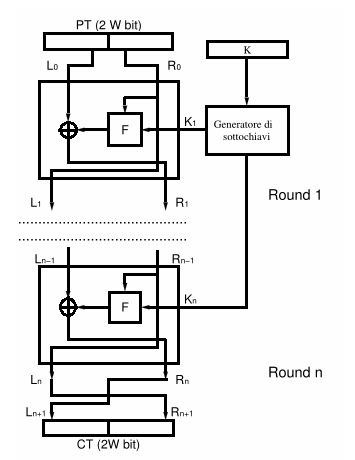
\includegraphics[width=\columnwidth]{img/feistel1}
						\caption{Encryption}			
					\end{figure}
				\end{center}
			\end{column}
			\begin{column}{0.7\textwidth}
				Il generico round $i-esimo$ di encryption può essere descritto come segue:
				$$Round(L_{i-1},R_{i-1},K_i) = (L_i,R_i)$$dove$$
				\begin{cases}
				L_i = R_{i-1} \\
				R_i = F(R_{i-1},K_i) \oplus L_{i-1}
				\end{cases}$$
			\end{column}
		\end{columns}
	\end{frame}

	\begin{frame}
		\frametitle{Schema}
		\begin{columns}
			\begin{column}{0.4\textwidth}
				\begin{center}
					\begin{figure}
						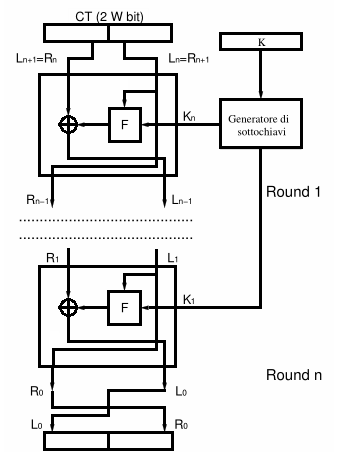
\includegraphics[width=\columnwidth]{img/feistel2}
						\caption{Decryption}			
					\end{figure}
				\end{center}
			\end{column}
			\begin{column}{0.7\textwidth}
				Per la decryption basta far passare il ciphertext dallo \tblue{stesso algoritmo} invertendo l'ordine delle sottochiavi. Infatti
				$$Round(R_{i},L_{i},K_i) = (R_{i-1},L_{i-1})$$ dove
				$$\begin{cases}
				R_{i-1} = L_i \\
				L_{i-1} = R_{i} \oplus F(R_{i-1},K_i) = R_{i} \oplus F(L_i,K_i)
				\end{cases}$$
			\end{column}
		\end{columns}
	\end{frame}

	\begin{frame}
		\frametitle{Cifrari di Feistel}		
		I parametri da scegliere sono quindi:
		\begin{itemize}
			\item Dimensione dei \tblue{blocchi}
			\item Dimensione della \tblue{chiave}
			\item Numero di \tblue{round}
			\item Algoritmo per generare le \tblue{sottochiavi}
			\item Funzione $\tblue{F}$
		\end{itemize}
	\end{frame}


	\section{DES}

	\begin{frame}
		\begin{center}
			\LARGE{\textcolor{blue}{I giorni nostri: Data Encryption Standard}}
		\end{center}
	\end{frame}

	\subsection{DES}
	
		\begin{frame}
			\frametitle{DES}		
			\begin{itemize}
				\item Sistema crittografico più usato \tblue{attuamente}
				\item Adottato dal \tblue{NIST} (National Institute of Standards and Technology) nel 1977
				\item Si tratta di una \tblue{variante} dei cifrari di Feistel
			\end{itemize}
		\end{frame}
	
		\begin{frame}
			\frametitle{Caratteristiche}		
			\begin{itemize}
				\item Plaintext diviso in blocchi di \tblue{64 bit}
				\item Chiave di \tblue{56 bit}
				\item \tblue{16} round
				\item Dalla chiave \tblue{vengono generate} le 16 sottochiavi da usare una ogni round
			\end{itemize}
		\end{frame}
	
		\begin{frame}
			\frametitle{Funzionamento}	
			\begin{columns}
				\begin{column}{0.4\textwidth}
					\begin{center}
						\begin{figure}
							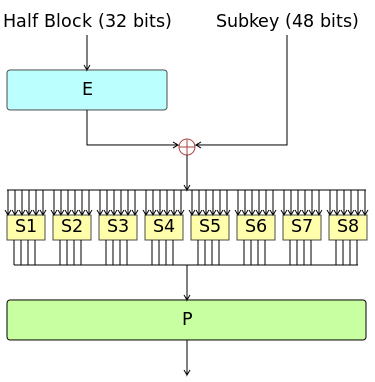
\includegraphics[width=\columnwidth]{img/des}
							\caption{Schema DES}
						\end{figure}
					\end{center}
				\end{column}
				\begin{column}{0.55\textwidth}
					\begin{itemize}
						\item Plaintext (64 bit) diviso a metà (come Feistel)
						\item E \tblue{"espande"} 32 bit portandoli a 48
						\item Viene fatto lo XOR con la \tblue{sottochiave}
						\item Si passa attraverso le \tblue{S-boxes}
						\item I 32 bit che escono dalle S-boxes entrano nella \tblue{P-box} che effettua l'ultima permutazione
					\end{itemize}
				\end{column}		
			\end{columns}		
		\end{frame}
	
		\begin{frame}
			\frametitle{S-boxes}	
			\begin{center}
				\begin{figure}
					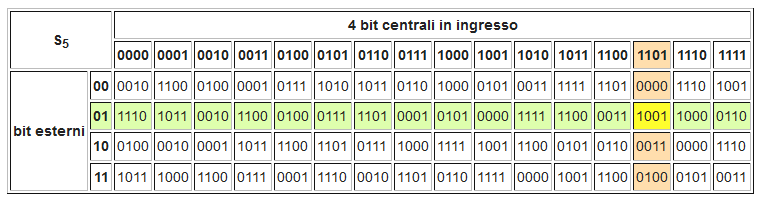
\includegraphics[scale=0.5]{img/desbox}
					\caption{Una S-box}
				\end{figure}
			\end{center}
			\begin{columns}
				\begin{column}{0.5\textwidth}
					\begin{itemize}
						\item \tblue{Input} 6 bit, output 4 bit
						\item Indice di riga i 2 bit più \tblue{esterni}
					\end{itemize}
				\end{column}
				\begin{column}{0.5\textwidth}
					\begin{itemize}
						\item Indice di colonna i 4 bit \tblue{centrali}
						\item \tblue{Output} i 4 bit nella casella selezionata
					\end{itemize}
				\end{column}
			\end{columns}
		\end{frame}
	
		\begin{frame}
			\frametitle{Sottochiavi}	
			\begin{columns}
				\begin{column}{0.3\textwidth}
					\begin{center}
						\begin{figure}
							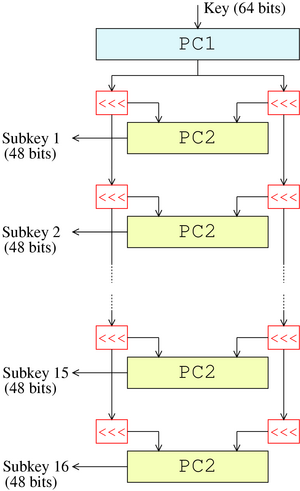
\includegraphics[scale=0.3]{img/deskey}
							\caption{Creazione delle sottochiavi}
						\end{figure}
					\end{center}
				\end{column}
				\begin{column}{0.65\textwidth}
					\begin{itemize}
						\item Selezione di 56 bit della chiave (8 sono di controllo)
						\item Divisi in due metà da 28 bit
						\item Shift a sinistra di 1 o 2 bit a seconda della sottochiave
						\item Selezione di 48 bit
					\end{itemize}
				\end{column}
			\end{columns}	
		\end{frame}
	
		\begin{frame}
			\frametitle{Resistenza}		
			\begin{itemize}
				\item La criptanalisi del DES è quella sulla quale sono state pubblicate \tblue{più informazioni} rispetto ad un qualunque altro algoritmo di cifratura a blocchi
				\item Presenta alcune \tblue{vulnerabilità teoriche} agli attacchi known-plaintext ma, per essere applicate, necessitano di conoscere $\approx 5\cdot10^{11}$ testi in chiaro scelti.
				\item L'\tblue{unico} attacco praticabile resta quello di forza bruta
				\item Attualmente si riesce a trovare la chiave in \tblue{poche ore}
			\end{itemize}
		\end{frame}
	
	\subsection{TripleDES}
	
		\begin{frame}
			\frametitle{Triple DES}		
			\begin{itemize}
				\item 3DES viene standardizzato per \tblue{applicazioni finanziarie} nel 1985
				\item Diventa parte del Data Encryption Standard nel \tblue{1999}
				\item Usa 3 chiavi (\tblue{non necessariamente distinte}) per effettuare tre diverse esecuzioni di DES
			\end{itemize}
		\end{frame}
	
		\begin{frame}
			\frametitle{Schema di funzionamento}		
			\begin{center}
				\begin{figure}
					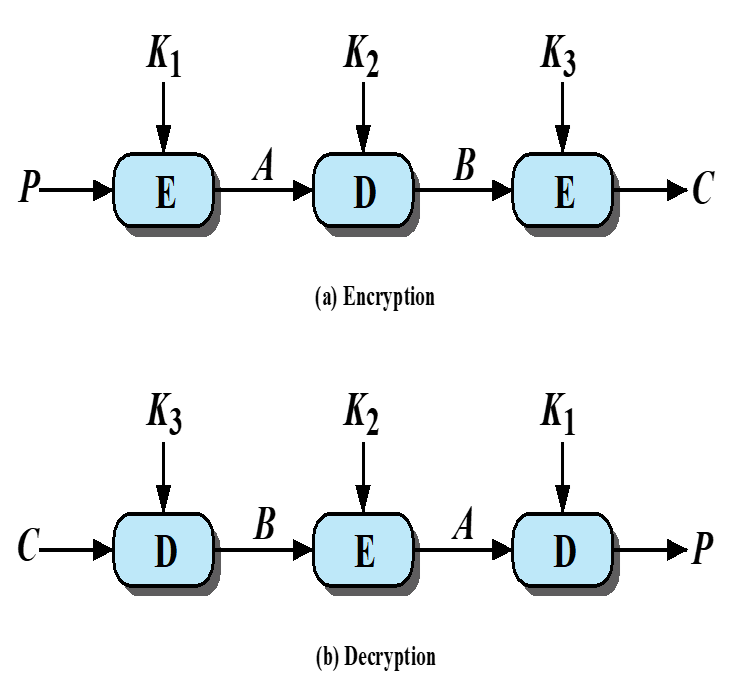
\includegraphics[scale=0.2]{img/tripleDes}
					\caption{Triple DES}
					$C=E(K_3,D(K2,E(K_1,P)))$\\
					$P=D(K_3,E(K2,D(K_1,C)))$
				\end{figure}
			\end{center}
		\end{frame}
	
		\begin{frame}
			\frametitle{Triple DES}		
			\begin{itemize}
				\item Usando sempre la \tblue{stessa} chiave otteniamo DES $$E(K_1,D(K_1,E(K_1,P)))$$
				\item Si possono usare \tblue{due chiavi distinte} e si usano nell'ordine $$E(K_1,D(K_2,E(K_1,P)))$$
				\item Con 3 chiavi distinte si arriva ad una lunghezza di 168 bit e \tblue{si escludono} gli attacchi di forza bruta $$E(K_3,D(K2,E(K_1,P)))$$
			\end{itemize}
		\end{frame}


	\section{AES}

	\begin{frame}
		\begin{center}
			\LARGE{\textcolor{blue}{La sicurezza non basta mai: Advanced Encryption Standard}}
		\end{center}
	\end{frame}

	\subsection{AES}
	
		\begin{frame}
			\frametitle{AES}	
			\begin{itemize}
				\item AES è stato standardizzato dal NIST nel \tblue{2001} in previsione di sostituire 3DES
				\item Implementa un algoritmo \tblue{Rijndael}
				\item Usa blocchi \tblue{128 bits}
				\item Lunghezza della chiave 128, 192 o 256 bits (in genere \tblue{128})
			\end{itemize}
		\end{frame}
	
		\begin{frame}
			\frametitle{Funzionamento}
			\begin{columns}
				\begin{column}{0.45\textwidth}
					\begin{center}
						\begin{figure}
							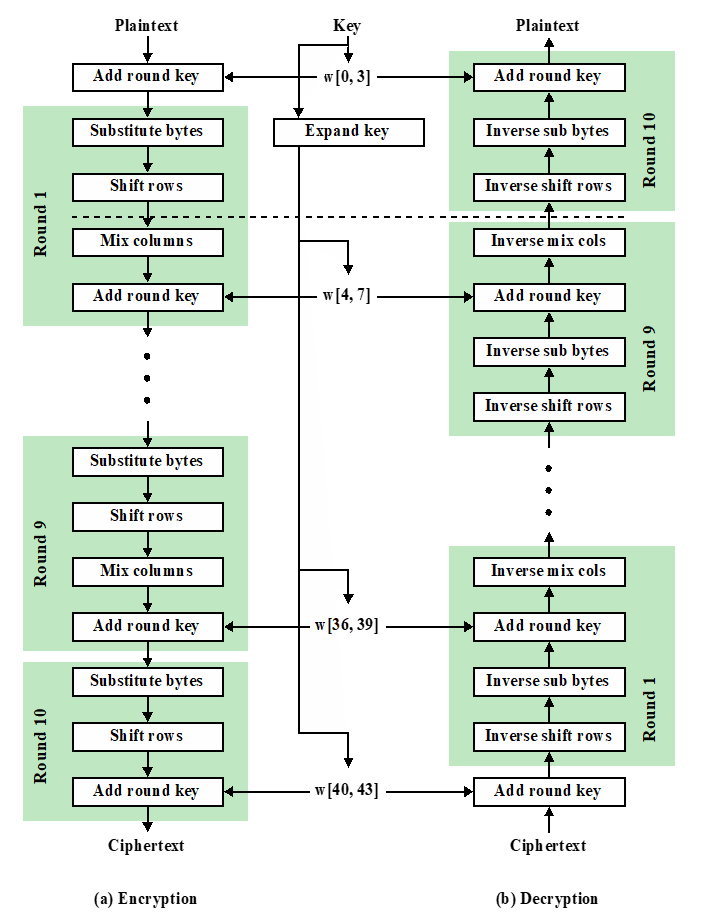
\includegraphics[width=\columnwidth]{img/aes}
							\caption{Algoritmo AES}
						\end{figure}
					\end{center}
				\end{column}
				\begin{column}{0.6\textwidth}
					\begin{itemize}
						\item Il blocco in input viene rappresentato come una matrice quadrata di bytes (4x4) chiamata \tblue{stato}
						\item Anche la chiave viene rappresentata come una matrice quadrata di bytes
						\item Il \tblue{gestore delle chiavi} ricava dalla chiave un array di 44 words da 4 byte che verranno usate come sotto-chiavi
						\item L'algoritmo si divide poi in \tblue{10 round caratterizzati} (tranne l'ultimo) da 4 fasi
					\end{itemize}
				\end{column}
			\end{columns}
		\end{frame}
	
	\subsection{Specifiche}
	
		\begin{frame}
			\frametitle{Sostituzione}
			\begin{columns}
				\begin{column}{0.45\textwidth}
					\begin{center}
						\begin{figure}
							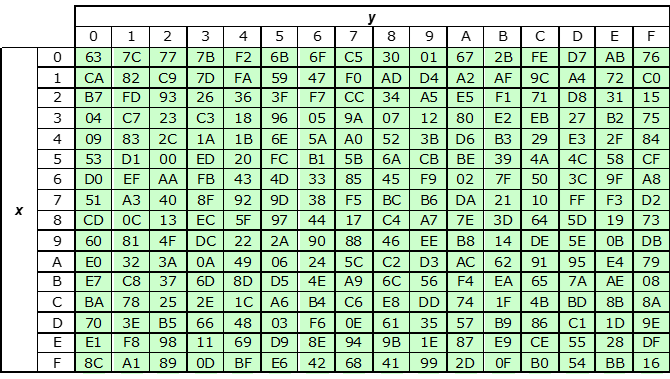
\includegraphics[width=0.8\columnwidth]{img/aesbox}
							\caption{AES S-Box}
						\end{figure}
						\begin{figure}
							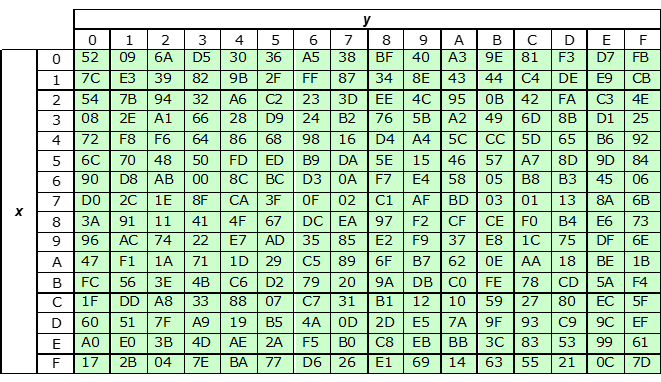
\includegraphics[width=0.8\columnwidth]{img/aesbox2}
							\caption{AES S-Box inversa}
						\end{figure}
					\end{center}
				\end{column}
				\begin{column}{0.7\textwidth}
					\begin{itemize}
						\item Sostituzione \tblue{byte per byte} attraverso la S-Box
						\item La S-Box usata è nota ed ha ottime proprietà di \tblue{non linearità}
						\item La S-Box è stata studiata a lungo per evitare che abbia \tblue{punti fissi} o \tblue{punti opposti}
					\end{itemize}
				\end{column}
			\end{columns}
		\end{frame}
	
		\begin{frame}
			\frametitle{Scostamento}
			\begin{center}
				\begin{figure}
					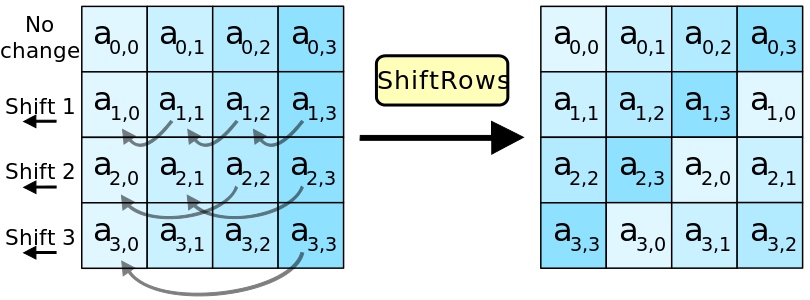
\includegraphics[scale=0.3]{img/shiftrow}
					\caption{Shift rows}
				\end{figure}
			\end{center}
			\begin{itemize}
				\item Scostamento delle righe \tblue{dipendente} dal numero di riga 
				\item L'ultima colonna diventa la \tblue{diagonale} della nuova matrice
			\end{itemize}
		\end{frame}
	
		\begin{frame}
			\frametitle{Mix columns}
			\begin{center}
				\begin{figure}
					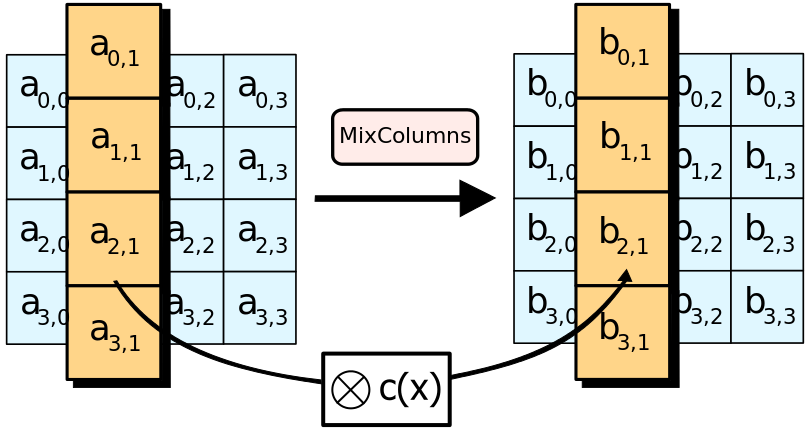
\includegraphics[scale=0.2]{img/mixcolumns}
					\caption{Mix columns}
				\end{figure}
			\end{center}
			\begin{itemize}
				\item Combinazione lineare \tblue{invertibile} delle colonne in funzione di tutti i 4 bytes di ogni colonna
				\item Insieme allo shift row applicano il criterio di \tblue{diffusione} e \tblue{confusione}
			\end{itemize}
		\end{frame}
	
		\begin{frame}
			\frametitle{Add round key}
			\begin{center}
				\begin{figure}
					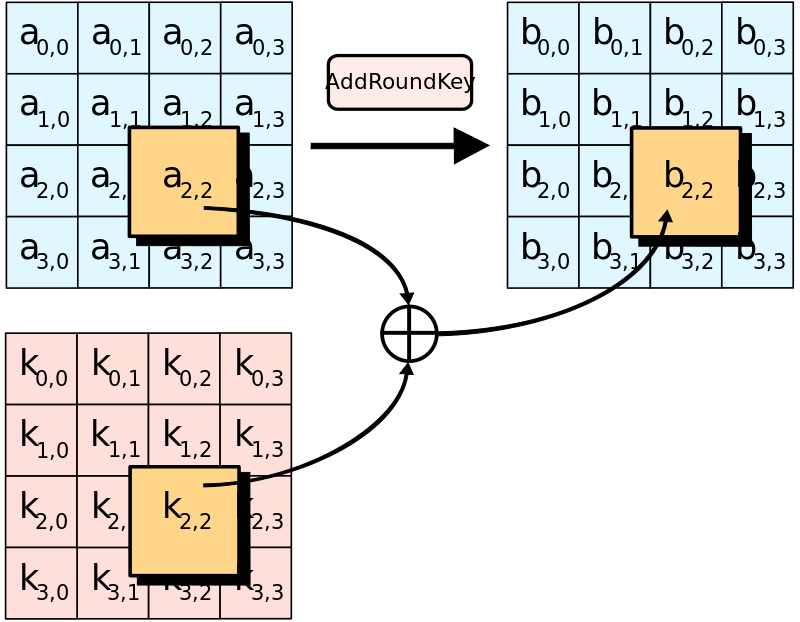
\includegraphics[scale=0.1]{img/addroundkey}
					\caption{Add round key}
				\end{figure}
			\end{center}
			\begin{itemize}
				\item \tblue{XOR} bit a bit dello stato attuale con la chiave di round
			\end{itemize}
		\end{frame}
	
		\begin{frame}
			\frametitle{Sicurezza}
			{
			\fontsize{10}{0}
			\begin{itemize}
				\item Semplice da implementare e richiede \tblue{poche risorse} (ottimo per le smart-card)
				\item NSA utilizza chiavi di 128 bits per crittografare documenti classificati \tblue{SECRET} e di 192 o 256 per i \tblue{TOP SECRET}
				\item \tblue{Distributed.net} ha effettuato il miglior attacco di forza bruta conosciuto su chiave da 64 bit impiegando circa 5 anni utilizzando potenza computazionale di volontari sparsi per il mondo
				\item Approfondita descrizione \tblue{matematica} riguardante AES solleva le maggiori preoccupazioni
				\item Nel 2002 l'attacco teorico \tblue{XSL} basato appunto su alcune proprietà matematiche ha mostrato un punto debole di AES. Computazionalmente non è applicabile.
			\end{itemize}
			}
		\end{frame}



	\section{RC4}

	\begin{frame}
		\begin{center}
			\LARGE{\textcolor{blue}{Dai blocchi allo stream: RC4}}
		\end{center}
	\end{frame}

	\subsection{Stream}
	
		\begin{frame}
			\frametitle{Stream cipher}		
			\begin{itemize}
				\item I cifrari a blocchi codificano input producendo output \tblue{un blocco alla volta}
				\item I cifrari a stream codificano l'input \tblue{costantemente} producendo output di volta in volta
				\item Generalmente si codifica \tblue{un byte} alla volta
				\item Necessita di un generatore di byte \tblue{pseudocasuali}
			\end{itemize}
		\end{frame}
	
		\begin{frame}
		\frametitle{Generatore pseudo-casuale}		
		\begin{itemize}
			\item Riceve in input la chiave e restituisce uno \tblue{stream} di byte pseudocasuali chiamato \tblue{keystream}
			\item Il keystream deve essere \tblue{impredicibile} senza conoscere la chiave
			\item Viene messo in XOR \tblue{bit a bit} con lo stream da cifrare
			\item Se lo stream fosse \tblue{veramente} casuale, otterremmo una sorta di One Time Pad
		\end{itemize}
	\end{frame}

	\subsection{RC4}
	
		\begin{frame}
			\frametitle{RC4}		
			\begin{itemize}
				\item Progettato nel 1987 da \tblue{Ron Rivest} per la RSA security
				\item Inizialmente la NSA lo aveva tenuto segreto ma fu diffuso anonimamente su internet nel \tblue{1994}
				\item Codifica \tblue{un byte} alla volta
				\item Il \tblue{periodo} del generatore pseudo-casuale è $\approx 10^{100}$
				\item Molto \tblue{veloce} (minimo 8 massimo 16 operazioni macchina per byte)
				\item Usato in SSL/TLS, lo \tblue{standard di comunicazione} tra browser e server
			\end{itemize}
		\end{frame}
	
		\begin{frame}
			\frametitle{Algoritmo}		
			\begin{itemize}
				\item Chiave a \tblue{lunghezza variabile}, da 1 a 256 bytes
				\item Con la chiave si inizializza il vettore di stato \tblue{S} di 256 bytes
				\item $S\left[ 0\right] , S\left[ 1\right] ,\dots,S\left[ 255\right] $ contengono una permutazione di \tblue{tutti} i numeri a 8 bit compresi tra 0 e 255
				\item Viene \tblue{scelto} un byte $S\left[ k\right] $ che viene usato per la encryption in modo sistematico
				\item Tutti i byte di S vengono \tblue{nuovamente permutati}
			\end{itemize}
		\end{frame}
	
		\begin{frame}
			\frametitle{Algoritmo}	
			\begin{columns}
				\begin{column}{0.65\textwidth}
					\begin{center}
						\begin{figure}
							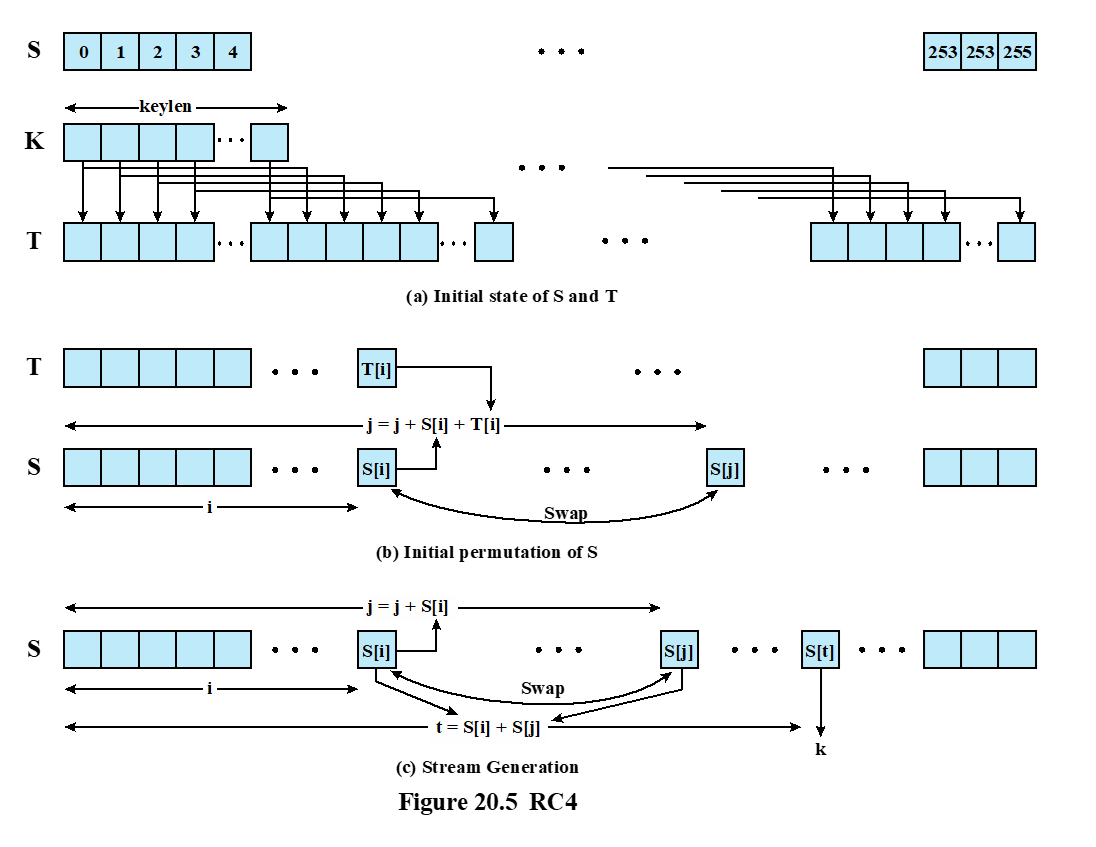
\includegraphics[width=\columnwidth]{img/rc4}
							\caption{Schema generale}
						\end{figure}
					\end{center}
				\end{column}
				\begin{column}{0.35\textwidth}
					\begin{center}
						\begin{figure}
							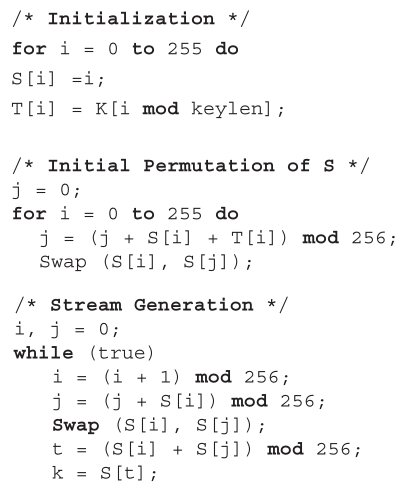
\includegraphics[width=\columnwidth]{img/rc4algo}
							\caption{Pseudocodice}
						\end{figure}
					\end{center}
				\end{column}
			\end{columns}	
		\end{frame}
	
	\subsection{Sicurezza}
		
		\begin{frame}
			\frametitle{(In)Sicurezza}	
			\begin{itemize}
				\item Molto semplice ma molto \tblue{debole}
				\item Il problema non è RC4 ma il \tblue{PRNG}
				\item Alta \tblue{periodicità} nei primi 256 bytes
				\item Forte \tblue{correlazione} tra chiave e keystream
			\end{itemize}
		\end{frame}
	
		\begin{frame}
			\frametitle{(In)Sicurezza}	
			\begin{itemize}
				\item Molte implementazioni eseguono un ciclo di 256 iterazioni \tblue{a vuoto} prima di utilizzare il keystream
				\item Mozilla \tblue{ha rimosso} da Firefox il supporto a RC4 dalla versione 44 (26 gennaio 2016)
				\item L'alternativa migliore attualmente è \tblue{SNOW} di Thomas Johansson e Patrik Ekdahl dell'università svedese di Lund
			\end{itemize}
		\end{frame}



	
	{ % all template changes are local to this group.
		\setbeamertemplate{navigation symbols}{}
		\begin{frame}[plain]
			\begin{tikzpicture}[remember picture,overlay]
			\node[at=(current page.center)] {
				
\includegraphics[scale=0.45]{img/All}
			};
			\end{tikzpicture}
		\end{frame}
	}

	\begin{frame}{Bibliografia}
		\begin{thebibliography}{99}
			
			\bibitem[Boreale]{p1} Michele Boreale (2012)
			\newblock \textit{Note per il corso di CODICI E SICUREZZA, UNIFI}
			
			\bibitem[Stallings, Brown]{p2} William Stallings, Lawrie Brown (2015)
			\newblock \textit{Computer security: principles and practice}
			
			\bibitem[]{p3} Francesca Merola (2014)
			\newblock \textit{Slides del corso di elementi di crittografia, UNIROMA3}
			
			\bibitem[Wikipedia]{p4} ENIGMA su Wikipedia
			{
				\fontsize{10}{0}
				\newblock \url{https://it.wikipedia.org/wiki/Enigma_(crittografia)}
			}
		
			\bibitem[Cryptomuseum]{p5} Cryptomuseum
			\newblock \url{https://www.cryptomuseum.com}
						
		\end{thebibliography}
	\end{frame}
	
	
\end{document}